
\doublespacing

\begin{titlepage}
	
	\begin{figure}[H]
		\centerline
		{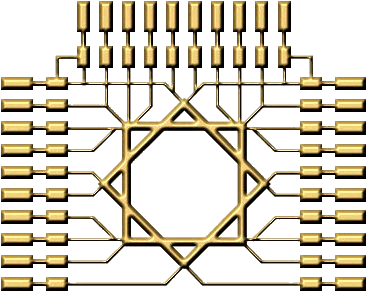
\includegraphics[width=0.2\linewidth]{images/HIAST_logo.png}}
		\label{}
	\end{figure}
	\begin{center}
		
		\large
		%\centering
		%\includegraphics[width=1\linewidth]{Figures/cover/HIAST.png}\\
		الجمهورية العربية السورية\\
		المعهد العالي للعلوم التطبيقية والتكنولوجيا\\
		قسم النظم الالكترونية
		\Large
		\vspace{3em}
		%\hline
		\vspace{3pt}
		%\hline
		\vspace{7pt}
		
		\textbf{
			الملاحقة بالاعتماد على تقنيات التعلم العميق\\
			\textLR{Visual Object Tracking Using Deep Learning Techniques}
		}
		\vspace{7pt}
		%\hline
		\vspace{3pt}
		%\hline
		
		
		\Large
		\vspace{1em}
		أعدت هذه الأطروحة لنيل\\
		درجة الماجستير في نظم  التحكم والروبوتيك\\
		
		
		\vspace{2em}
		\textbf{
			إعداد:\\
			م. مي عبود \\
			\vspace{2em}
			إشراف:\\
			د. آصف جعفر
			\hspace{4em}
			د. عمر حمدون\\
		}
		\vspace{4em}
		كانون الأول $ 2022 $
	\end{center}
	\begin{center}
		\textbf{إهداء}\\
		أهدي هذا العمل إلى أمي ...
		\newline
		وإلى روح أبي ...
		
	\end{center}
\end{titlepage}
\newpage

\newpage
\begin{center}
	\textbf{كلمة شكر}\\
أتوجه بالشكر الجزيل لكل من ساهم في إنجاح هذا العمل, وأخص بالذكر الدكتور آصف جعفر والدكتور عمر حمدون لما قدماه من وقت وجهد في الإشراف على البحث. 
\end{center}


